\section{Optimization Under Uncertainty}

\begin{figure}[H]
    \centering
    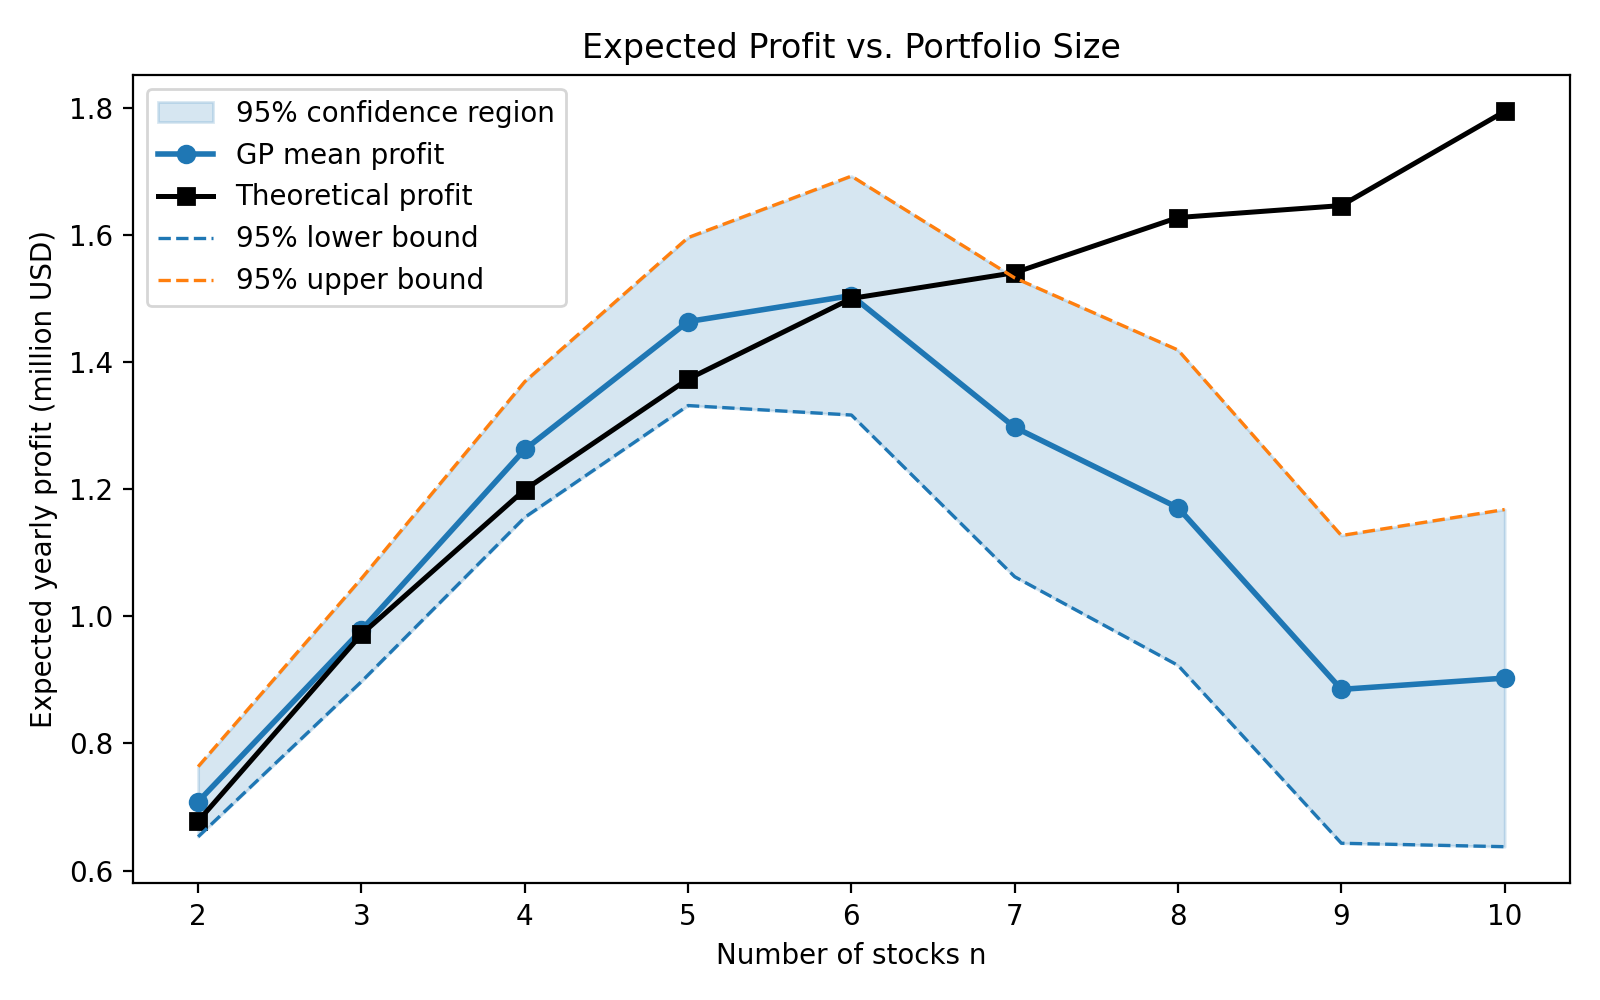
\includegraphics[width=0.9\linewidth]{img/expected_profit_vs_n.png}
    \caption{Expected yearly profit as a function of portfolio size.}
\end{figure}

\subsection*{Recommendation}

The recommended portfolio size is $n=6$. Using only the theoretical
diversification curve, the largest expected yearly profit occurs at $n=10$,
because adding more stocks increases the gross return term even though the
minimum separation distance decreases. However, the Gaussian-process model
learned from the simulation data gives a more conservative efficiency estimate
at small separations. Under the GP posterior mean, the best expected profit is
at $n=6$, about \$1.50M per year.

The uncertainty bounds support the same general decision. The lower 95\%
confidence bound is maximized at $n=5$, while the upper 95\% confidence bound is
maximized at $n=6$. This means the main tradeoff is between $n=5$ and $n=6$:
$n=5$ is slightly more conservative, but $n=6$ has the best posterior-mean and
optimistic performance. Therefore, I would choose $n=6$ unless the manager is
strongly risk averse, in which case $n=5$ is the safer alternative. Additional
simulation effort should focus near the corresponding distances
$p^\star \approx 4.0$ and $p^\star \approx 4.7$, where the decision is most
sensitive to uncertainty.

% \begin{enumerate}[label=(\alph*)]
    % \item Following the theoretical efficiency curve, the best portfolio size is $n=10$.
    % \item Based on the prediced GP posterior mean, the best portfolio size is $n=6$ as it maximizes the expected profit.
    % \item Yes. With the lower 95\% confidence bound, the best size is $n=5$. In the plot the expected profit this point is just above $n=6$.
    % \item With the upper 95\% confidence bound, the best portfolio size is $n=6$.
    % \item Designing to the mean is good for a neutral decision maker, the lower bound is appropriate for a risk-averse manager, and the upper bound is appropriate when the manager is willing to accept more uncertainty.
    % \item Additional simulations should be collected near $p \approx 4.0$ and $p \approx 4.7$, because these distances correspond to the competing $n=5$ and $n=6$ recommendations where uncertainty can change the decision.
% \end{enumerate}

\subsection*{Code}

The implementation is included in \hyperref[expected_profit]{Appendix~\ref*{expected_profit}}.
 
